\chapter{Analysis}
\section{Requirements and Constraints}
\subsection{Requirements}
\begin{itemize}
    \item Search and selection of hardware components.
    \item Software design.
    \item PCB design.
    \item 5S outer shell 3D design.
    \item Actual product realization.
    \item Laboratory tests.
\end{itemize}
\subsection{Constraints}
\begin{itemize}
    \item The project must be presented for avaluation within deadline.
    \item The project has to be valitated at the ocean.
    \item The pretended autonomy has to be of a mouth at minimum.
\end{itemize}
\section{State of the art}
\subsection{Economy}
\subsection{Ecology}
\subsection{Sports}
\section{Market Research}
\section{System Architecture}


\subsubsection{Block Diagram}

\begin{figure}[H]
    \centering
    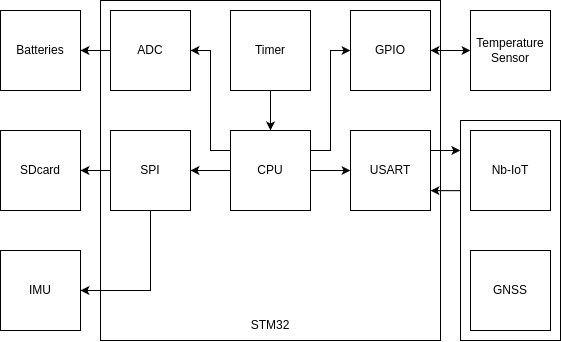
\includegraphics[width=0.7\textwidth]{images/diagrams/block_diagram/block_diagram_1/block_diagram.drawio.png}  % Adjust the width as necessary
    \caption{Block Diagram}
    \label{fig:Block Diagram}        
\end{figure}

\subsubsection{Use Case}

\begin{figure}[H]
    \centering
    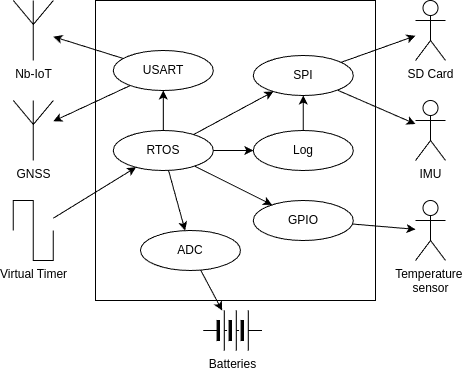
\includegraphics[width=0.7\textwidth]{images/diagrams/use_case/Use Case.drawio.png}  % Adjust the width as necessary
    \caption{Use Case Diagram}
    \label{fig:Use Case Diagram}        
\end{figure}

\subsubsection{Sequence Diagram}

\begin{figure}[H]
    \centering
    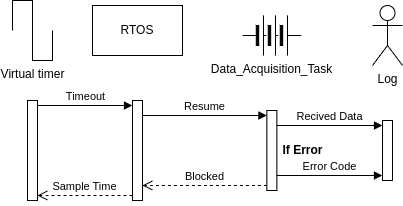
\includegraphics[width=0.7\textwidth]{images/diagrams/sequence_diagram/sequence_diagram_1/Sequence Diagram.drawio.png}  % Adjust the width as necessary
    \caption{Sequence Diagram of Sensor Task}
    \label{fig:Sequence Diagram of Sensor Task}
\end{figure}

\begin{figure}[H]
    \centering
    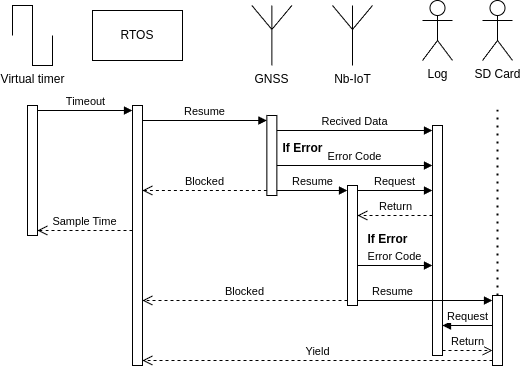
\includegraphics[width=0.7\textwidth]{images/diagrams/sequence_diagram/sequence_diagram_2/Sequence Diagram.drawio.png}  % Adjust the width as necessary
    \caption{Sequence Diagram for Sending and Archive Task}
    \label{fig:Sequence Diagram for Sending and Archive Task}        
\end{figure}

\subsubsection{Threads} 
Once this problem requires a list of taks to be executed, using a OS will allow
a better project organization and performance with little to no impact in power consumption.

As the ST uC offers a variety of RTOS, the implementation will be acessible with good support due to the
CMSIS v2 abstraction layer.

The division in Threads demands a separation in Priority levels, as the OS scheduler takes in consideration 
once both tasks are ready for execution.  

Seting a task priority it must take in vision the resources the task will use, the time it will take to execute said behavior
and the actual importance in matching it time constraints. In order to menage this level of complexity, the RTOS offers a set of
tools for tasks control that will be used for its sincronization and comunication.

\subsubsection{High Priority Threads}
Tasks that will handle the outer communication as GNSS and the internet integration will take the higher priority once, as will be handled
by a peripheral, it execution will be faster, only using the USART interface for AC trasmission. 

\subsubsection{Normal Priority Threads}
The only task here will be the one that has enough inportance to be prioritised over the sensors but as the transmission beggins it should release the processor
for the outer communication.

\subsubsection{Low Priority Threads}
Tasks that only has to measure the sensors ocasualy and have no problem to be removed from the CPU execution
once their execution is, in their majority, assyncronos.

%rescrever
\begin{figure}[H]
    \centering
    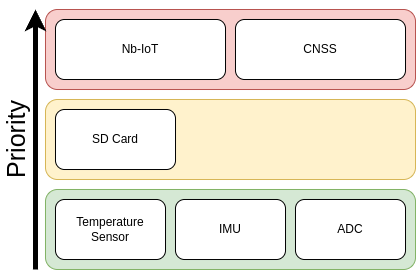
\includegraphics[width=0.7\textwidth]{images/diagrams/threads/thread.drawio.png}  % Adjust the width as necessary
    \caption{Thread Priority Stack}
    \label{fig:Thread Priority Stack}        
\end{figure}


\begin{figure}[H]
    \centering
    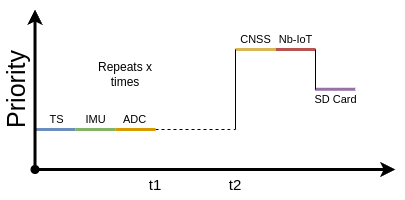
\includegraphics[width=0.7\textwidth]{images/diagrams/threads/graph/threads_graph.drawio.png}  % Adjust the width as necessary
    \caption{Thread Temporal Graph}
    \label{fig:Thread Temporal Graph}        
\end{figure}